\chapter{Metallurgy}
\label{chap:metallurgy}
\section{Introduction}
We shall begin this section with some quotes from the masters.
Cottrell, for his part, observed that 
metallurgy would require a ``theory... which explains
the properties of metallic solids and the explanation of the origin of this
structure from the structures of individual atoms." Similarly in Vol. 35
Heine noted ``What we lack is a fundamental quantum theory of the cohesion
and structure of a wide diversity of solids." 
The development of such a theory must heed the early warning of Wigner and Seitz: 
"If one had a great calculating machine, one might 
apply it to the problem of solving the Schr\"odinger equation for each metal
and obtain thereby the interesting physical quantities... It is not clear, however,
that a great deal would be gained by this. Presumably the results would agree
with the experimentally determined quantities... It would be preferable instead
to have... a simple description of the essence of the factors which determine cohesion
and an understanding of the origins of variation in properties from metal to metal."\cite{wigner55}.

The previous chapters, though hopefully enjoyable in their own right, 
were really just meant to bring us to the stage where we can start 
using the principles of locality and recursion methods to compute 
the structural and 
mechanical properties of extended solids. 

This chapter will focus on determining which properties and trends we would like
to calculate and how to go about calculating them.

%Perhaps the most interesting aspect of physical metallurgy is how
%macroscopic parameters can be directly connected to the solution of 
%the wave equation governing the atomic scale motion of the electrons.
%Feynman's definition of a chemical bond.
%It now becomes quite clear why the strongest and most important attractive 
%forces arise when there is a concentration of charge between two nuclei. 
%The nuclei on each side of the concentrated charge are each strongly attracted to it.
%Thus they are in effect attracted towards each other. 
%
\section{A Condensed Historical Interlude}
The calculation of the cohesive energy and lattice constant of 
metallic sodium\cite{wigner34a, wigner33,wigner34b}.
by Wigner and Seitz can be viewed as the initiation of the field
of theoretical materials science.

Subsequent work in this field by Fuchs extended Wigner and Seitz's analysis
to the cohesive and elastic properties of monovalent metals \cite{fuchs35, fuchs36} 
Around the same time quantum theory was being
applied to explain the appearance of different phases in alloys in terms 
of Brillouin zones \cite{bethe29, bouckhaert36, owen33, jones34}. 

Born's work provides the standard treatment of 
the stability of lattices to short and long wavelength
vibrations by considering general analytic forms for the interatomic potentials\cite{born40,born42},
with other workers again making extensions of the theory to particular
lattice types \cite{power41, nabarro52}. The work of Brockhouse, which led to the 1994
Nobel Prize in Physics, and others on neutron spectroscopy provided striking 
experimental confirmation of the predicted properties of lattice vibrations\cite{brockhouse62}.

With the rise of, what Friedel called the `computational lobby', the prospect 
of obtaining numerical solutions to the wave equations governing the motion of 
electrons in solids began to appear increasingly attractive. It is at this
point the two, increasingly divergent, schools of thought in electronic structure
come in to focus. On the one hand workers, amongst them Hubbard and Pettifor \cite{ziman65, hubbard67, pettifor69} sought
to rationalize trends in the transition metals with a minimal analytic models capable of 
capturing the physical mechanisms dictating the observables. These efforts were in parallel 
with workers obtaining numerical solutions to the wave equations \cite{andersen75, jepsen75}
Friedel wrote a paper emphasising the complimentary usefulness of the two schools of thought
\cite{friedel73}.

Towards the end of the 1970s the first systematic tests of local density 
functional based methods in a metallurgical context began to appear.
It appeared that the methods were capable of obtaining \cite{moruzzi77, gelatt77}. 
particularly satisfying agreement with experimental data available for 
cohesive energies, bulk moduli, and equilibrium nuclear separation across 
the transition metal series.

\section{Crystal Structure}
In keeping with the unifying theme of the book the targeted quantities
will first be described and formulated in general terms and then mapped
on to a set of recursion calculations. From these calculations it will be
shown that we can compute the preferred crystal structures and the vibrational and 
elastic properties of many transition metals from the perspective of the 
local atomic environment.

As a final demonstration of the recursion method in the context of metallurgy 
we apply the calculations to a particular model for embrittlement. This
will set us up nicely for the next (and final) chapter when we apply
recursive techniques to determine more macroscopic parameters. 

Step number uno in the field of theoretical metallurgy is a theory that correctly
describes the crystal structures formed by different pure metals. 
Often the first three lattices encountered by students of metallurgy 
will be FCC, HCP, and BCC.

\begin{quote}
‘Close-packing’ lacks a unique meaning without a specification of 
what is being packed, and what is meant by close and, in particular, 
what is close to what. The thinking underlying the citation of f.c.c. 
and h.p.c. as examples of closest-packed structures is the packing of 
equal hard spheres. A metal is not an assembly of hard spheres,but rather of 
nuclei and electrons.These are both corpundular, with nowhere vanishing 
wavefunctions, but because of their very large mass ratio it is an excellent 
approximation to consider the nuclei as located at points
but the electrons as forming a continuum, with density throughout the metal 
everywhere positive and, except close to the nuclei, quasi-uniform.
\end{quote}

The closeness of close packed structures stems from trying to squeeze
the largest number of atoms into a particular volume
with a hard lower bound on the approach of the nuclei.
The BCC structure solves a different problem in that it finds a
distribution of nuclei likely to be closest to the electrons.

Early considerations based on orbital hybridisation and geometry
were performed by Altmann, Coulson, and Hume-Rothery who treated 
the problem in Ref.~\cite{altmann57}. One of the earliest triumphs 
of the recursion method was the sorting of the Lave 
Phases \cite{haydocklaves75,johannes76} into distinct structures. 
%Density functional studies of the crystal phases \cite{chan86,paxton97}

The ability of the tight binding framework
to provide an explanatory model for trends in homologous materials is
well demonstrated by the Pettifor's work on the transition
metal series \cite{pettifor70}, the Chevrel 
compounds of Molybdenum chalcogenides Ref.~\cite{bullet77}.
and the structures of the compounds in the Lave phases 
in Ref.~\cite{johannes76}.

\section{Crystal Properties: A Momentous Triumph}
For a metallurgist the first set
of homologous series we would like to explain is
the structures formed by the elementary transition metals
and a quantitative theory of the defect energetics in the
close packed materials.
In this section we will employ the moments formulation of 
the tight binding method to rationalize the behaviour of
BCC and close packed crystals (See.\ref{sec:relatedmethods}).
At the end of the section a number of computational excercises
are set in order to compare the theoretical predictions
with experimental data.

In Fig.~\ref{fig:fccvshcp} the two close packed structures 
Face Centered Cubic and Hexagonal Close packed are compared.
\begin{figure}
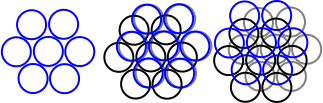
\includegraphics[scale=1.0]{./metallurgy/closepacked.pdf}
\caption{The close packed structures and the different stacking patterns
in the hexagonal close packed and face centered cubic crystals.\label{fig:fccvshcp}}
\end{figure}

In Fig.~\ref{fig:fcchcppaths} the paths contributing to the 
\begin{figure}
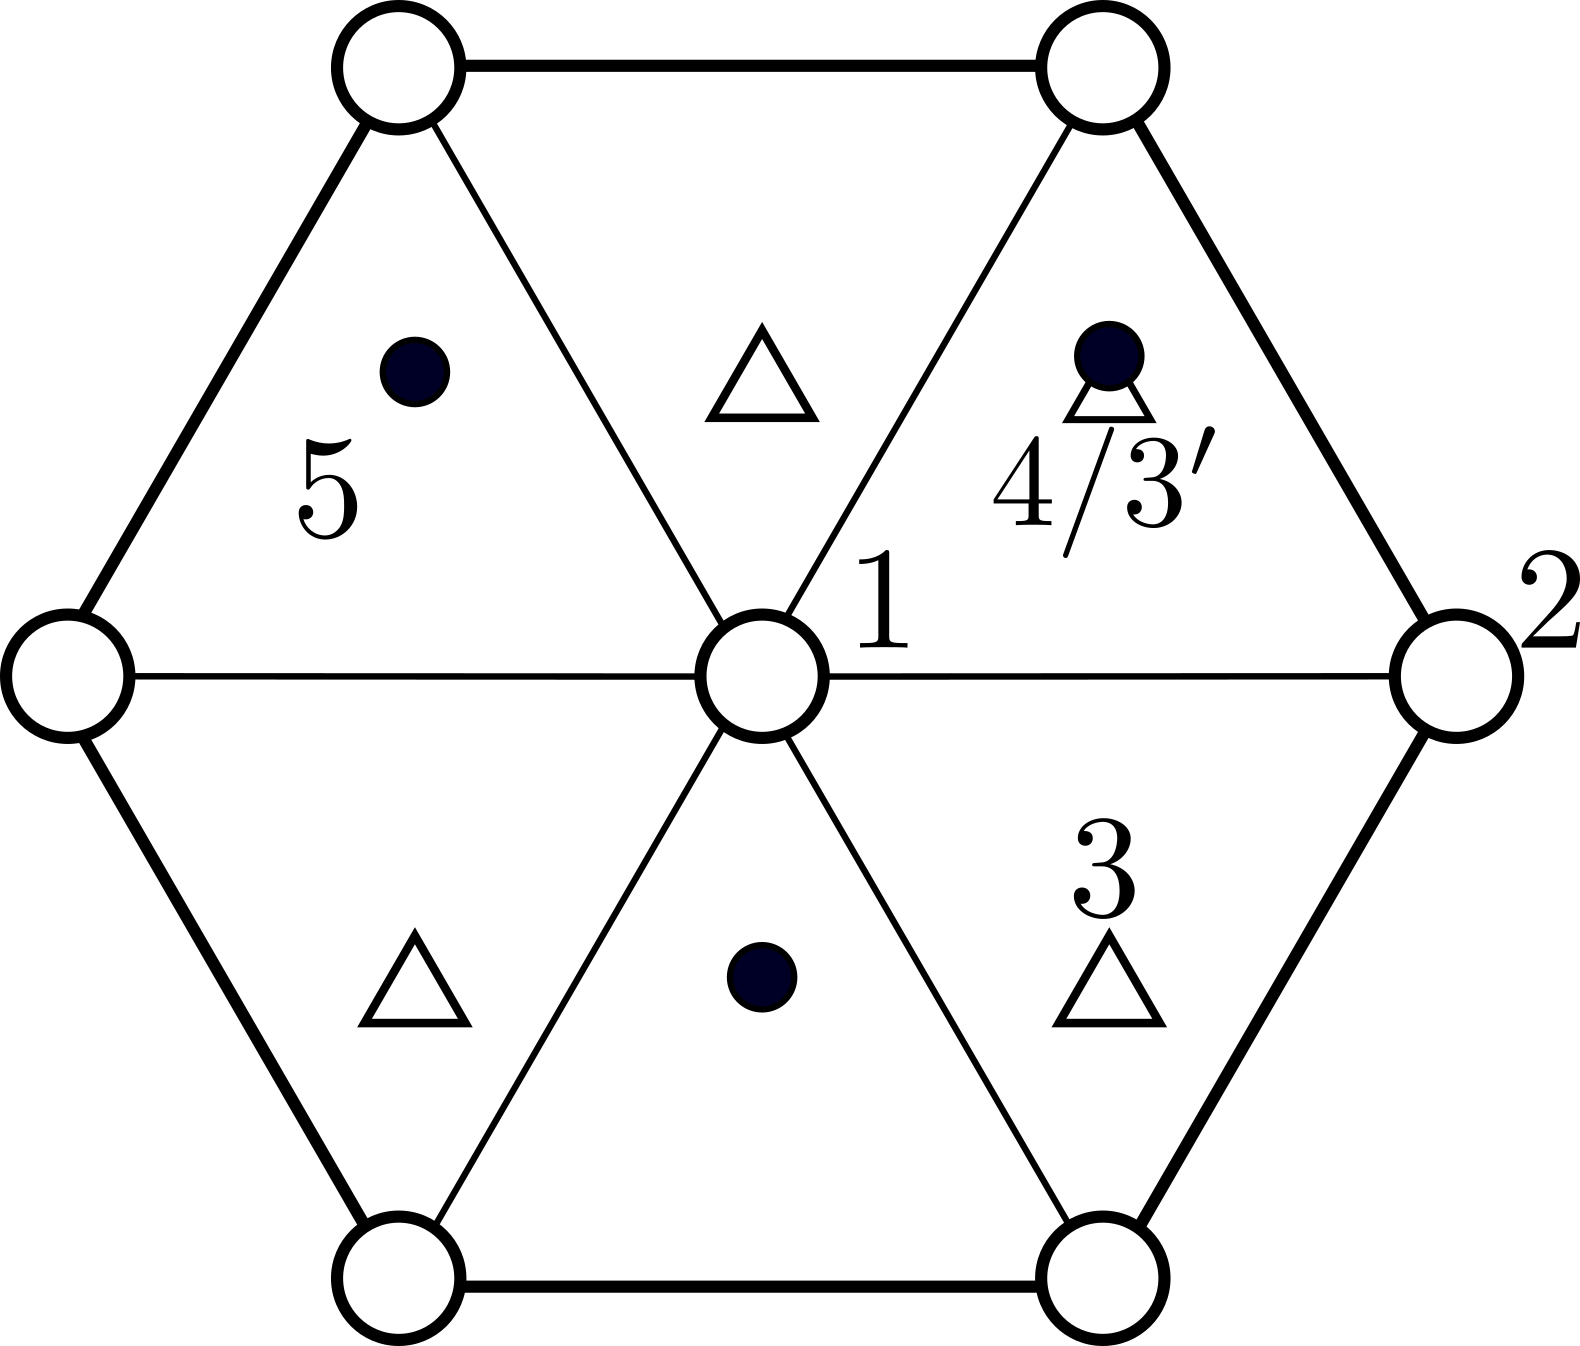
\includegraphics[scale=1.0]{./metallurgy/fccvshcppaths.png}
\caption{$\mu_{4}$ The paths involving three neighbouring planes 
in the fcc lattice can be separated into three types: 
Type I: 1-3-1-5-1, Type II: 1-3-2-4-1, Type III:1-3-1-4-1.
The equivalent HCP paths can be obtained by substituting 
$3\rightarrow 3'$. After: Ducastelle and 
Cyrot-Lackmann~\cite{ducastelle71}. \label{fig:fcchcppaths}}
\end{figure}

%\exercise{Using the recursion library examine the energy differences in the HCP, BCC, and FCC 
%structures. The recursion method allows us to obtain numerically stable results, 
%reasoning in terms of chains and moments gives us physical insight.}

\subsection{$c/a$ Ratio in Hexagonal Close Packed Metals}

\subsection{Stacking Faults}
%
The stacking sequences can get mixed up from time to time
in the close packed materials.o
%
\begin{table}
\begin{tabular}{c c c}
Defect Type  &  F.C.C.     &  H.C.P.  \\
intrinsic  &  ABCBCA     &  BABCACA   \\  
extrinsic  &  ABCBABC    &  AABCABA  \\ 
twin       &  ABCBAC     &  BABCBC   \\
\end{tabular}
\caption{The different stacking fault types in close packed lattices.\label{tab:stackingfaults}}
\end{table}

\section{Lattice Vibrations}
%insight into \cite{varma79a, varma79b}.

\section{Elastic Tensors}
Shearing, straining, Young's modulus, poisson ratio, elastic tensors these are the
stuff of every undergraduate materials mechanics course.
Imagine you have some tensor $\epsilon$ and you apply a virtual pure strain to a collection atoms.

The present section will demonstrate how to compute some of the elastic properties
of a BCC crystal using recursion techniques. We will look at two approaches.
One of them involves looking at the changes in the total energy with
respect to a deformation of the lattice and picking out the 
second derivative of this change, which, depending on the deformation chosen,
will correspond to an element of the elastic tensor. The second approach
proceeds directly from the Hamiltonian that has been chosen and employs second order
perturbation theory to calculate the contributions of
the interatomic force constants to the elastic tensor. 
The second approach has some distinct numerical 
and conceptual advantages.

\subsection{The Expressions We Need}
In the author's opinion elasticity is made difficult by the appearance of a variety
of numerical prefactors. An abundance of factors of 2,
1/3, 1/6, etc. seem to arise in the course of a calculation hindering progress. 
We will not attempt to give an introduction to the principles of elasticity rather
we would just provide a collection of equations and some visuals 
that relate deformations of the crystal to changes in total energy.

In this section we shall specialize the analysis to a cubic crystal, specifically a body centered cubic
crystal and simply state the lattice deformations which are required to probe the 
different material elastic constants. We will follow the notation given by Finnis where
a much more detailed exposition can be found along with pointers to comprehensive references.

The first constant we might calculate is the Bulk Modulus which is defined:
%
\begin{equation}
\label{eq:bulkmodulus}
B\equiv V_{c} \frac{\partial^{2} E}{\partial V_{c}^{2}}
\end{equation}
%
that is the second order variation in the energy with respect to changes in the 
sample volume multiplied by the volume. After some rearrangement (which is a useful
exercise) Eq.~\ref{eq:bulkmodulus} can be written:
%
\begin{equation}
V_{c}\frac{\partial^{2} E}{\partial V_{c}^{2}} = \left[-\frac{2}{3}\frac{\partial E}{\partial V_{c}}+\frac{1}{9V_{c}}\frac{\partial^{2}E}{\partial \gamma^{2}} \right],
\end{equation}

where gamma is a scalar that can be varied and controls the change in volume:
%
\begin{equation}
V_{c}(\gamma) = (1+\gamma)^{3}V_{c}(0)
\end{equation}
%

The elastic energy contribution to a sample is written:
%
\begin{equation}
\label{eq:eq:elasticenergy}
E^{elastic} = \frac{1}{2}C_{11}(\epsilon^{2}_{1} + \epsilon^{2}_{2} + \epsilon^{2}_{3}) + C_{12}(\epsilon_{1}\epsilon_{2}
+\epsilon_{2}\epsilon_{3} + \epsilon_{3}\epsilon{1}) + C_{44}(\epsilon^{2}_{4} + \epsilon^{2}_{5} + \epsilon^{2}_{6})
\end{equation}
%
where Voight's notation ($\epsilon_{1}=\epsilon_{xx}$...) has been used. Staring at Eq.~\ref{eq:elasticenergy} you
should be able to see that deformations which pick out only $C_{44}$ or $C_{11}$ should be fairly easy to write down
however $C_{12}$ requires a little more work to pick out on its own.

Let $\epsilon_{ij} = \gamma T_{ij}$, (we like introducing $\gamma$ because it is useful to have a simple scalar
to parametrize the lattice distortions which are written as a matrix $T$).
We can now write the modified lattice constants as:
%
\begin{equation}
R'_{i\alpha} =  R_{i\alpha} + \gamma \sum_{\beta} T_{i\beta}R_{i\beta}
\end{equation}
%

Following Finnis we rewrite Eq.~\ref{q:elastic energy} in terms of the T matrices:

To obtain the shear elastic constant: $C' = \frac{1}{2}(C_{11}-C_{12})$ the following deformation
matrices are particularly helpful a tetragonal distortion:
%
\begin{equation}
T^{t} =  
    \begin{bmatrix}
         1 &   0   & 0  \\
         0 &  -0.5 & 0  \\    
         0 &   0   &-0.5 
    \end{bmatrix}
\end{equation}

or a distortion of the (110) plane:
%
\begin{equation}
T^{(110)} = 
    \begin{bmatrix}
            1 &  0 & 0  \\
            0 & -1 & 0  \\    
            0 &  0 & 0 
    \end{bmatrix}
\end{equation}

To obtain the $C_{44}$ contributions we may introduce
a rhombohedral distortion:
%
\begin{equation}
T^{(111)} =  
    \begin{bmatrix}
             0   & 0.5 & 0.5 \\
             0.5 & 0   & 0.5 \\    
             0.5 & 0.5 & 0 
    \end{bmatrix}
\end{equation}
%
or a (100) distortion:
%
\begin{equation}
T^{(100)} =  
\begin{bmatrix}
             0 & 1 & 0 \\
             1 & 0 & 0 \\    
             0 & 0 & 0 
\end{bmatrix}
\end{equation}
%

For any new potential the computation of the predicted elastic properties should
be the first port of call. For the crystal to be stable $B,C',C_{44}$ must all be
greater than 0 so that gives a definite sanity check on the model. 

Let us apply these deformations to a BCC crystal and see what comes out.
First we make a few observations. The deformation matrices for
$C'$ will not change the relative positions of the first nearest neighbours.
This deformation will, however, alter the second nearest neighbour positions so we may expect
that the $C'$ shear will be largely determined by the second nearest neighbour interactions. 
As for the $C_{44}$ distortions all neighbours participate in a rhombohedral distortion
and all neighbours save the two second nearest neighbours orthogonal to the $(100)$
plane participate in a $T^{(100)}$ distortion. 

If we wish to approximate the second derivative of the total energies with 
respect to $\gamma$ we are going to have to be careful. We won't be able
to obtain it by doing a single total energy difference calculation. That
will not contain enough information. We could obtain an estimate by assuming
an expression of the form: 
%
\begin{equation}
\Delta E(\epsilon) = 2\epsilon^{2} E^{(2)} + \epsilon^{4} E^{(4)},
\end{equation}
%
and solving for $E^{(2)}$. Or we could do multiple energy calculations for 
a sequence of distortions and fit a polynomial to the results extracting
the second difference from the polynomial fit.

If you have worked your way through Sec.~\ref{sec:vibrations} you might already have
a set of force constant pairs to hand. In that case Eq.~\ref{eq:brockhouselimit} will give you
another means of obtaining the required elastic constants.
%
\begin{equation}
\label{eq:brockhouselimit}
C_{i} = \frac{1}{B_{i}a}\sum_{n} n^{2}\Phi_{n}
\end{equation}
%
The correspondence between the elastic constant $C_{i}$ and the phonon modes is given
in Table~\ref{tab:brockhouse}:

\begin{table}
\begin{center}
\begin{tabular}{|c|c|}
\hline
Phonon Branch  & Elastic Constant \\
\hline
(00q)L  & $C_{11}$ \\
(00q)T  & $C_{44}$ \\
(qqq)L  & $(C_{11}+2C_{12}+4C_{44})/3$ \\
(qqq)T  & $(C_{11}-C_{12}+C_{44})/3$ \\
(qq0)L  & $C_{11}+2C_{12}+4C_{44}$ \\
(qq0)T1 & ($C_{11}$ - $C_{12}$)/2\\
(qq0)T2 & $C_{44}$\\
\hline
\end{tabular}

\caption{Correspondence of phonon branches with combinations of elastic constants.}
\end{center}
\end{table}

Notice that the factor of $n^{2}$ means you have to be quite confident in the accuracy of
the force constants connecting distant pairs of atoms. Otherwise any error
in your calculation will be rapidly amplified as you move to more distant neighbours. 
The force constants must be decaying with some alacrity 
(perhaps at least as quickly as $n^{-4}$) in order for this to be a numerically convergent
approach.

\subsection{Local Stress Fields}
The TBB Model \cite{nielsen83, sutton88} gives us a means of defining and calculating 
a local in the sense of a per atom stress tensor. If $I$ and $J$ 
are cartesian components $x,y,z$ to first order in the energy:
%
\begin{equation}
\delta E^(1) = \sum_{I} \sum_{(ij)}\Omega^{i}\sigma^{i}_{IJ}\epsilon_{IJ}
\end{equation}
%
The contribution to the IJ component of the stress tensor is:
%
\begin{equation}
\label{eq:atomstress}
\sigma^{i}_{IJ} = \frac{1}{\Omega^{i}}\sum_{j\neq i}\sum_{\alpha\beta}G(\epsilon)_{i\alpha j\beta}\frac{\partial H_{j\beta i\alpha}}{\partial R_{jI}}(R_{jJ}-R_{iJ})
\end{equation}
%
The pair contributions can be added to obtain the full stress tensor. 
But if we are only interested in the electronic contributions
Eq.~\ref{eq:atomstress} is already good enough
for an application of the local stress tensor,
see Ref.~\cite{ohta90}

%As usual we need to know the $R$ dependence of our
%integrals, both hopping and on-site, which we went to the trouble 
%of learning in Chapter~\ref{chap:wannier}.
%Ref.~\cite{terakura84} demonstrates how the recursion method
%may be used to compute the elastic constants of a material.

The interaction of dislocations and defects reveals one of the most difficult problems
in theoretical materials science: the coupling of long range elastic fields
with local chemical changes. This coupling of length scales makes
reliable quantitative calculations difficult. Variations in the electronic structure
induce strains in the metal matrix which feed back into the electronic structure. 
It appears that one requires a theory with quantum accuracy on the scale of an 
interatomic bond that simultaneously takes into account the long range elastic 
field.

%To proceed we will assume we can obtain a relaxed structure where all the atomic forces are
%in equilibrium. We then follow the derivation of Ref.~\cite{freedman09} which uses the free energy
%of the system at equilibrium to derive a tensor that describes the interaction of point defects 
%with elastic fields. A few different ways of computing this tensor are then described \cite{nazarov16}.
%The force method of computing the elastic dipole tensor lends itself 
%immediately to the expressions introduced all the way back in 
%Chapter~\ref{chap:invariance}, Eq.\ref{eq:tbforce}. \cite{paxton90}.

\section{Recursing through Defects and Dislocations}
The ability of the recursion method to quantify the local changes in interatomic bonding and
forces makes it a particularly useful tool for the study of dislocations. 

Understanding the interaction of interstitials and impurities with the motion of
dislocations through a crystal is a central goal of theoretical metallurgy with
with work on this subject beginning in the 1950s \cite{cochardt55}.

The local density of states for atoms at a screw dislocation core have been computed by \cite{paidar81,masuda81}. 
The change in the local bonding picture induced by a vacancy in Fe was examined in Ref.~\cite{masuda82,ohta87}.

\section{Grain Boundaries}
The analysis of Read and Shockley in Ref.~\cite{read50} serves as a comprehensive
introduction to the field of interfaces in condensed matter. The modern
standard reference on the subject of interfaces in materials is Sutton and 
Baluffi Ref.~\cite{sutton95}.

A number of experimental probes are capable of detecting the presence of 
grain boundaries but efficient and accurate means of determining 
the orientation relationships between grains remains an outstanding problem.
For an analysis of the statistic arrangement of grains using quaternion
algebra see Ref.~\cite{sutton96}.
%structural unit model \cite{sutton89} random interfaces?
The possibility of examining grain boundaries atomistically has interested
researchers since it became practical to perform atomistic simulations
with realistic potentials see Refs.~\cite{bristowe75,wolf83,paxton87,paxton88,paxtonsutton88,
kohyama88,kohyama94,paxton96,rittner96,tschopp07,momida13,du11,du12,mceniry18} for a
snapshot of the way computational studies of interfacial structure 
has evolved over time.

\subsection{Discrete Boundary Dislocation Networks}
Combining isotropic elasticity with discrete dislocation networks
we can gain some useful practice in contour integration and arrive
at a closed set of expressions for strains in linear elasticity
theory next to a large angle grain boundary. 

These expressions are given in Ref.~\cite{sutton95} and derived here.

\subsubsection{Analytic Treatment of Strain Fields}
\label{gbalgebra}
%Just for reference, the algebra is similar for all other components of the stress, and
%can be extended to cases where we have a traveling edge dislocation i.e. instead of
%a sum over n $n$ we have a factor like (y-vt)....
First we introduce the function:
%
\begin{equation}
f(z) =  \pi\cot(\pi z)\frac{(Y-z)(3x^{2} + (Y-z)^{2})}{(X^{2} + (Y-z)^{2})^{2}}.
\end{equation}
%
This has simple poles at $z = 0, \pm 1, \pm 2,...$. It also has two 2nd 
order poles at  $z_{1}=iX+Y$, $z_{2}=-iX+Y$. The residue at $z_{2}$ can
be found from the following expression: 
%
\begin{equation}
{\rm Res}(z_{2}) = \lim_{z\rightarrow z_{2}}\frac{d}{dz}(z-z_{2})^{2}
\frac{\cot(\pi z)(Y-z)(3X^{2}+(Y-z)^2)}{(z-z_{1})^{2}(z-z_{2})^{2}}.
\end{equation}


\begin{align}
\label{eq:2ndstep}
{\rm Res}(z_{2})&=\frac{\pi^{2}}{\sin^{2}(\pi z_{2})}\left[\frac{(Y-z_{2})(3x^{2}+(Y-z_{2})^{2})}{(z_{2}-z_{1})^{2}}\right]\\
  &+\frac{\pi\cot(\pi z_{2})}{(z_{2}-z_{1})^{2}}\left[-(3x^{2} + (Y-z_{2})^{2})-2(Y-z_{2})^{2}\right] \\
  &+\frac{2\pi\cot(\pi z)(Y-z_{2})(3X^{2}+(Y-z_{2})^{2})}{(z_{2} - z_{1})^{3}}.
\end{align}
%
The second term in Eq.~\ref{eq:2ndstep} evaluates to zero and the remaining terms can be simplified to:
%
\begin{equation}
{\rm Res}(z_{2}) = \frac{\pi}{4\sin^{2}(\pi(Y-iX))}(i\pi X - \sin(2\pi(Y-iX))).
\end{equation}
%
The residue at $z_{1}$ can be found in a similar manner.

If we construct a set of contours as depicted in Fig.~\ref{fig:polediagram}.
\begin{figure}[!tbp]
\begin{center}
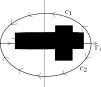
\includegraphics[scale=1.0]{./metallurgy/stresspolediagram.pdf}
\caption{Contours to determine sum. The lines of poles from the $\cot(\pi z)$ 
factor can be equated to the difference of the two 
second order residues.\label{fig:polediagram}}
\end{center}
\end{figure}

We can write down the sum as the difference of the two second order residues.

\subsubsection{Jordan's lemma}
We must consider the behaviour of the function $f(z)$ on the countours carefully in order to determine their contribution to the $\oint f(z) dz$ as we expand the semi-circular contours out to $\infty$.  Jordan's lemma says if we are able to write $f(z) = \exp(iaz)g(z)$ for positive $a$ then an upper-bound for the integral over the semi-circular contour in the upper-half plane is given by
%
\begin{equation}
\left|\int_{C_{1}}f(z)dz\right| \leq \frac{\pi}{|a|}\text{max}_{\theta\in [0,\pi]}\left|g(Re^{i\theta})\right|.
\end{equation}
%
A similar results holds for the lower-half plane, provided we now make $a<0$.  We now consider expansions for $\cot(\pi z)$:
%
\begin{eqnarray}
\cot(\pi z)&=&-i(e^{i2\pi z}+1)(1-e^{i2\pi z})^{-1}=-i(1+e^{i2\pi z})(1+e^{i2\pi z}+e^{i4\pi z}+\ldots)\label{eq:upper}\\
&=&i(1+e^{-i2\pi z})(1-e^{-i2\pi z})^{-1}=i(1+e^{-i2\pi z})(1+e^{-i2\pi z}+e^{-i4\pi z}+\ldots)\label{eq:lower}.
\end{eqnarray}
%
Focusing first on the upper-half plane we replace $\cot(\pi z)$ with equation~\ref{eq:upper}.  
Since $g(z)=f(z)/\cot(\pi z)$ goes to zero as $z\rightarrow\infty$ we can apply Jordan's 
lemma and ignore the contributions on $C_{1}$ from all positive powers of $e^{i2\pi z}$.  
However we still need to consider the $-i$ term, where Jordan's lemma doesn't apply.  
Substituting $z=Re^{i\theta}$ and taking the limit as $R\rightarrow\infty$ we obtain:
\begin{equation}
\int_{C_{1}}f(z)dz = \int_{\theta=0}^{\pi}d\theta iRe^{i\theta}*\frac{(i\pi R^{3}e^{3i\theta}}{R^{4}e^{4i\theta}} = -\pi^{2}.
\end{equation}
We now instead focus on $C_{2}$ and replace $\cot(\pi z)$ with equation~\ref{eq:lower}.  
Once again Jordan's lemma allows us to ignore the powers of $e^{-i2\pi z}$.  
However we still need to focus on the $i$ term.  Substituting $z=Re^{i\theta}$ and 
taking the limit as $R\rightarrow\infty$ we obtain:
%
\begin{equation}
\int_{C_{2}}f(z)dz = \int_{\theta=2\pi}^{\pi}d\theta iRe^{i\theta}\times\frac{(-i\pi R^{3}e^{3i\theta})}{R^{4}e^{4i\theta}} = -\pi^{2}.
\end{equation}

Let $I=\int_{\Gamma_{1}}f(z)dz$, then closing on the upper-half plane we have:
%
\begin{equation}
I-\pi^{2} = 2\pi i\left[Res(z_{1})+\sum_{n=-\infty}^{\infty}Res(z=n)\right].
\end{equation}
%
While closing on the lower-half plane gives:
%
\begin{equation}
I-\pi^{2} = -2\pi i Res(z_{2}),
\end{equation}
%
the negative sign arising because the contour goes clockwise on the lower-half plane.

\subsection{Dislocation-Interstitial Interactions}
Coupling of the hydrogen defects to the screw and edge dislocations can be
handled via the approach taken in \cite{cochardt55}.
The interaction energy between a dislocation and an interstial atom can
be calculated from the work done by moving each face of a cell a distance
$d_{i}$ against a force $F_{i}$ exerted by the stress field:
%
\begin{equation}
U_{DC} =+\sum_{i}F_{i}d_{i}.
\end{equation}
%
If the components of the stress tensor are assumed constant along the distance $a$
this energy can be written:
%
\begin{equation}
U_{\rm{DC}} = -(T_{D},S_{H})a^{3}= -\sum_{ik} \sigma_{ik}^{D}\epsilon^{H}_{ik} a^{3}.
\end{equation}
%

The observed slip system in $\alpha$-Fe for a screw dislotion is along the [111]
direction. Away from the dislocation core a bulk cell can be found and defined
with three unit vectors [100], [010], [001]. This unit cell is drawn in
Fig.~\ref{fig:interstitialcoords} (a). For an edge dislocation the slip plane is
assumed to be in the $(0\bar{1}1)$-plane, the dislocation line is in the direction
$\langle 211 \rangle$, and a Burgers vector in the direction $\langle \bar{1}11 \rangle$.

\begin{figure}[!tbp]
\begin{center}
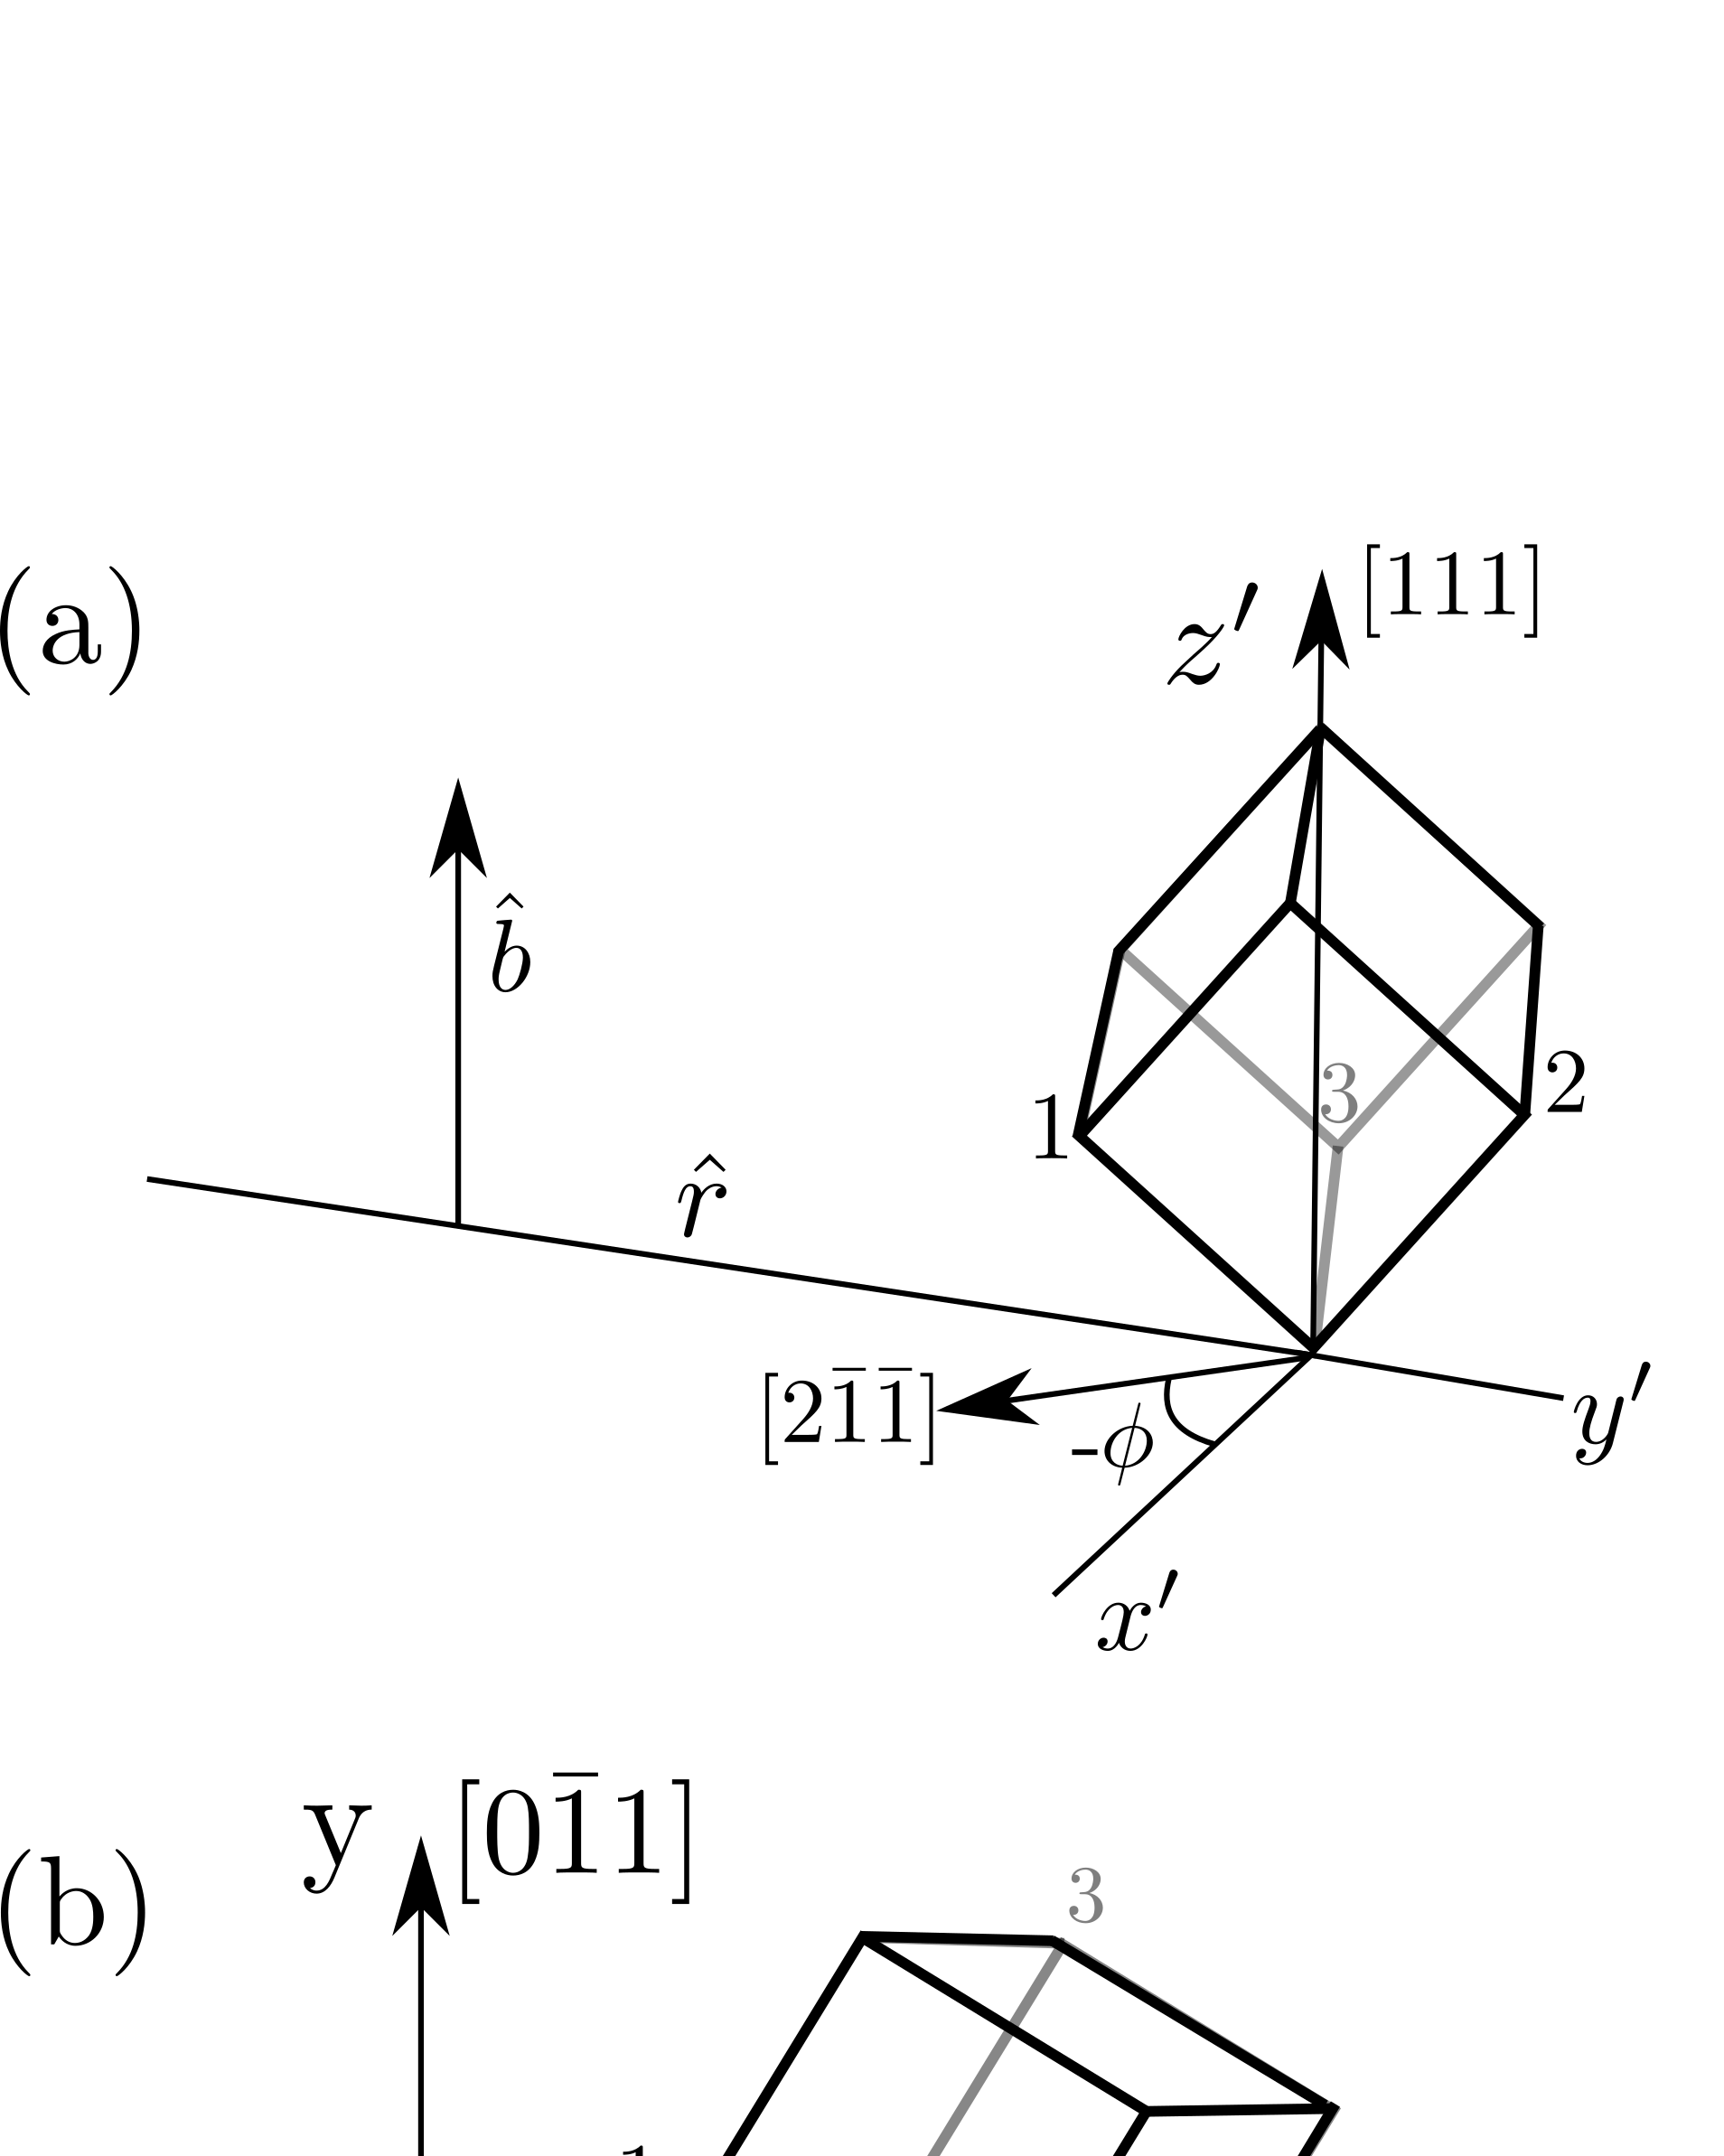
\includegraphics[scale=0.8]{./metallurgy/screwcoordinate.png}
\caption{\label{fig:interstitialcoords} Reproduced from \cite{cochardt55}.}
\end{center}
\end{figure}
%
In the analysis of Cochardt they calculate the interstitial-dislocation
energy for the defect atom, Carbon, at a distance $b$. In each case we
wish to translate the defect strain tensor into the

This can be accomplished by determining the transformation matrix $\mathbf{R}$:
which is the inverse of the matrix constructed by stacking up
the basis vectors in the new coordinate system,
%
\begin{equation}
\epsilon'_{ij} = \mathbf{R} \epsilon_{ij} \mathbf{R}^{\rm T}.
\end{equation}
%
In \cite{cochardt55} the strain tensor for a carbon atom in
a conventional rectangular unit cell for BCC iron is:
%
\begin{equation}
\left(
\begin{array}{ccc}
 a & 0 & 0 \\
 0 & b & 0 \\
 0 & 0 & c  \\.
\end{array}
\right),
\end{equation}
%

The stress tensor in the vicinity of a screw dislocation:
%
\begin{equation}
T^{x',y',z'}_{D}=
\frac{Gb}{2\pi r}
\left(
\begin{array}{ccc}
0 & 0 & 1 \\
0 & 0 & 0 \\
1 & 0 & 0 \\,
\end{array}
\right)
\end{equation}
%
and the stress tensor in the vicinity of an edge dislocation:
\begin{equation}
T^{x',y',z'}_{D}=
\frac{Gb}{2\pi(1-\nu)r}
\left(
\begin{array}{ccc}
-\sin\psi(1+2 \cos^{2}\psi) & \cos\psi\cos 2\psi & 0 \\
\cos\psi\cos 2\psi & \sin\psi\cos 2\psi & 0 \\
0 & 0 & -2\nu\sin\psi \\
\end{array}
\right).
\end{equation}
%
where the components of the tensor are estimated from X-ray measurements
of the tetragonal distortion of martensite to be $\epsilon_{a}=0.38$,
$\epsilon_{b}$=$\epsilon_{c}$=-0.026. For the screw dislocation
geometry given in Fig.~\ref{fig:interstitialcoords} (a) the transformed strain
tensor is:
%
%
\begin{equation}
\mathbf{\epsilon}'=\left(
\begin{array}{ccc}
 \frac{1}{3}[a+2 b+(a-b) \cos (2 \theta)] & -\frac{1}{3} (a-b) \sin (2 \theta ) & \frac{\sqrt{2}}{3} (a-b)\cos(\theta )\\
 -\frac{1}{3} (a-b) \sin (2 \theta ) & \frac{1}{3} (a+2 b+(b-a) \cos (2 \theta )) & -\frac{\sqrt{2}}{3}(a-b) \sin (\theta )\\
 \frac{\sqrt{2}}{3} (a-b) \cos (\theta ) & -\frac{\sqrt{2}}{3}(a-b)\sin(\theta ) & \frac{1}{3}(a+2 b)\\
\end{array}
\right).
\end{equation}
%
For the edge dislocation the inner product of the basis vectors does not vary with $\theta$
and the transformed strain tensor is given as:
%
\begin{equation}
\mathbf{\epsilon}'=\left(
\begin{array}{ccc}
 \frac{1}{3} (a+b+c) & \frac{c-b}{\sqrt{6}} & \frac{-2 a+b+c}{3 \sqrt{2}} \\
 \frac{c-b}{\sqrt{6}} & \frac{b+c}{2} & \frac{c-b}{2 \sqrt{3}} \\
 \frac{-2 a+b+c}{3 \sqrt{2}} & \frac{c-b}{2 \sqrt{3}} & \frac{2}{3}a + \frac{1}{6}(b+c) \\
\end{array}
\right).
\end{equation}

\section{Conclusion}
In this chapter we have looked at a number of the important quantities that
arise in metallurgy and how the recursion method is ideally suited to their 
computation. The motion of dislocations, the structure of grain boundaries, 
and alloying. 

